\documentclass[11pt]{article}

%--------------------------------------------------
% PACKAGES
%--------------------------------------------------
\usepackage[margin=1in]{geometry}
\usepackage{amsmath,amssymb}       
\usepackage{graphicx}              
\usepackage{hyperref}             
\usepackage[numbers]{natbib}      
\bibliographystyle{plainnat}       

%--------------------------------------------------
% TITLE
%--------------------------------------------------
\title{Removing Noise from Chaotic Dynamical Systems To Improve Accuracy of Takens Embedding and HAVOK}
\author{Igor Świerlikowski \\
	Maastricht University \\
	\texttt{i.swierlikowski@student.maastrichtuniversity.nl}}
\date{\today}

\begin{document}
	\maketitle
	
	%--------------------------------------------------
	% ABSTRACT
	%--------------------------------------------------
	\begin{abstract}
		This report explores the process of denoising chaotic dynamical systems and demonstrates the use of Takens Embedding and the HAVOK method for reconstructing and analyzing its dynamics. I propose a method for removing noise from chaotic signals and test the approach on the Lorenz Attractor system. My experiments show how some denoising techniques can be applied to minimize the impact of noisy measurements on our final reconstructed time delayed attractor.
	\end{abstract}
	
	%--------------------------------------------------
	% 1. INTRODUCTION
	%--------------------------------------------------
	\section{Introduction}
	Chaotic dynamical systems are prevalent in many fields, including physics, biology, and engineering. Despite them being fully deterministic, chaos arises due to sensitive dependence on initial conditions, leading to behavior that appears random and is difficult to predict over long time horizons. One approach to characterizing such complexity is the Hankel Alternative View of Koopman (HAVOK) method \citep{brunton2017}, which tries to decompose complex nonlinear systems into a mostly linear framework with a separate nonlinear forcing terms. This decomposition can then be used for easier forecasting and analysis.
	
	In practice, measurement noise is often unavoidable when studying chaotic systems. While such noise can't influence the underlying dynamics of a system, it is extremely difficult to describe using linear methods often "blinding" them. Consequently, efficient denoising techniques are critical for accurately reconstructing and predicting the true dynamics of these systems.
	
	In this report, we focus on one main technique for analyzing chaotic systems:
	\begin{itemize}
		\item \textbf{HAVOK Method}: A data-driven approach for decomposing time series into dominant modes and dynamical features. HAVOK begins with a time-delay Hankel matrix (as part of Takens Embedding) and applies Singular Value Decomposition (SVD) to said matrix. Afterwards, it uses Sparse Identification of Nonlinear Dynamics (SINDY) \citep{brunton2015} to represent the system with a main linear component and a separate nonlinear forcing term.
	\end{itemize}
	
	When this method is combined with a suitable denoising strategy, we can recover essential features of the underlying chaotic dynamics and potentially forecast intermittent events, such as lobe switching in the Lorenz system.
	
	%--------------------------------------------------
	% 2. METHODOLOGY AND EXPERIMENTS
	%--------------------------------------------------
	\section{Methodology and Experiments}
	
	\subsection{Data Description}
	In these experiments, I work exclusively with the Lorenz system, given by the following set of ordinary differential equations:
	\begin{equation}
		\begin{aligned}
			\frac{dx}{dt} &= \sigma (y - x),\\
			\frac{dy}{dt} &= x(\rho - z) - y,\\
			\frac{dz}{dt} &= xy - \beta z,
		\end{aligned}
		\label{eq:lorenz}
	\end{equation}
	where the classical parameter set is
	\[
	\sigma = 10, \quad \rho = 28, \quad \beta = \frac{8}{3}.
	\]
	For the experiments, the Lorenz system is evolved from \(t_0 = 0\) to \(t_1 = 50\) with a time step \(\Delta t = 0.001\). The initial conditions are set to \((x, y, z) = (-8, 8, 27)\). Numerical integration is carried out in MATLAB using the \texttt{ode45} solver with a strict error tolerance of \(10^{-12}\).
	
	To simulate measurement imperfections, Gaussian noise is added to the time series \emph{after} the system evolution is completed, thus modeling realistic sensor or measurement errors rather than influencing the underlying dynamics directly.
	
	\subsection{Noise Removal Techniques}
	Three primary methods are evaluated for noise removal:
	\begin{itemize}
		\item \textbf{Moving Average}: A simple method with only one parameter (\emph{window size}) which takes the average of surrounding measurements to smooth the data.
		\item \textbf{Savitzky--Golay}: Instead of simply averaging, this method fits a low-degree polynomial to a set of neighboring points, thus preserving features like local maxima and minima better than a simple moving average.
		\item \textbf{Wavelet Denoising} \citep{luo2012}: This approach uses the Discrete Wavelet Transform, a technique similar to the Fourier Discrete Transform but instead of fitting sine and cosine waves, it uses wavelets instead. This separates the signal into components of different frequencies. Noise is usually concentrated in higher frequencies, so thresholding or cutting off the high-frequency components can effectively reduce noise while preserving the main structure of the signal.
	\end{itemize}
	These methods were selected to cover a range of filtering techniques and to evaluate their relative performance in preserving the chaotic structure while reducing noise. Each method’s parameters were optimized across multiple noise samples to ensure a fair comparison between them.
	
	\subsection{Takens Embedding}
	Takens Embedding creates a delay-embedded attractor from time series data. In the HAVOK framework, this method is used by constructing a Hankel matrix of time-delayed coordinates. Following \citep{brunton2017}, we choose:
	\begin{itemize}
		\item An embedding dimension (number of rows in the Hankel matrix) of 100.
		\item A delay time of 0.001, matching the numerical integration time step.
	\end{itemize}
	
	\subsection{HAVOK Method}
	Once the Hankel matrix is formed, we perform SVD, yielding matrices \(U\), \(\Sigma\), and \(V^T\). Let \(\mathbf{v}(t)\) denote the relevant row components of \(V\). In the HAVOK procedure:
	\begin{itemize}
		\item We select the first \(r\) rows of \(V\) (i.e., the most dominant modes). Typically, \(r=15\) is used.
		\item Then sparse regression (SINDY) is applied to the first \(r-1\) rows, while the \(r\)-th row is treated as an intermittent forcing term.
	\end{itemize}
	Hence, we arrive at a nearly linear system of the form:
	\begin{equation}
		\frac{d}{dt}\mathbf{v}(t) = A\,\mathbf{v}(t) + B\,v_r(t),
		\label{eq:havok}
	\end{equation}
	where \(A\) and \(B\) are matrices identified through sparse regression, and \(v_r(t)\) is the last mode representing nonlinear forcing.
	
	\subsection{Error Measure}
	To evaluate reconstruction performance, we compare the \(\mathbf{V}\) matrix of the true or target system to the \(\mathbf{v}_{\text{sim}}\) matrix (the reconstruction). A straightforward approach I used is:
	\begin{equation}
		\text{error}_x = \sqrt{\sum \Bigl( V_x(t_{\text{span}},1{:}r) - v_{\text{sim}}(t_{\text{span}},1{:}r) \Bigr)^2 },
	\end{equation}
	where we sum over the relevant time points and dominant modes. However, as discussed later, this measure can be misleading because HAVOK does not treat all modes equally.
	
	\subsection{Experimental Procedure}
	Overall, the experiments follow this pipeline:
	\begin{enumerate}
		\item \textbf{Data Generation}: Numerically integrate the Lorenz system over \([0,50]\) using \(\Delta t = 0.001\).
		\item \textbf{Noise Addition}: Inject Gaussian or uniform noise after integration.
		\item \textbf{Denoising}: Apply one of the chosen noise removal techniques (Moving Average, Savitzky--Golay, or Wavelet).
		\item \textbf{Takens Embedding \& HAVOK}: Construct the Hankel matrix, perform SVD, and apply SINDY to form the HAVOK model.
		\item \textbf{Analysis}: Compare the reconstructed attractors, measure predictive performance, and assess sensitivity to noise.
	\end{enumerate}
	
	%--------------------------------------------------
	% 3. RESULTS
	%--------------------------------------------------
	\section{Results}
	
	\subsection{Investigating the Cause of Poor Performance}
	My first experiment added a small amount of noise (\(\text{sd} = 0.01\)) to the Lorenz system. As we can see in Figure~\ref{fig:figure1}, the delay-embedded attractor (Takens Embedding) itself looks almost the same, and the main differences appear when we linearize with HAVOK. This indicates that the problem arises in the linearization step, not in Takens Embedding.
	
	\begin{figure}[htbp]
		\centering
		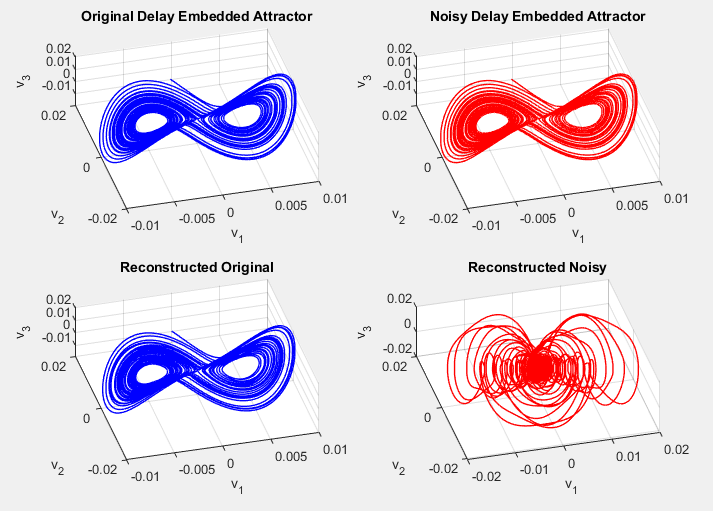
\includegraphics[width=0.7\linewidth]{Figure3}
		\caption{Comparing the original/noisy delay-embedded attractors and their reconstruction (small noise, \(\text{sd}=0.01\)). The top panels show the embedded attractors (original vs. noisy), whereas the bottom panel show the HAVOK restructions.}
		\label{fig:figure1}
	\end{figure}
	
	\subsection{Noise Removal Performance}
	Next, I applied Gaussian noise (sd = 0.01) to the Lorenz data and tested each denoising technique. Figure~\ref{fig:figure2} shows the time-series (the \(x\) variable versus time), including the noisy and denoised signals, while Figure~\ref{fig:figure3} shows a bar chart of the average RMSE across multiple trials for each method.
	
	\begin{figure}[htbp]
		\centering
		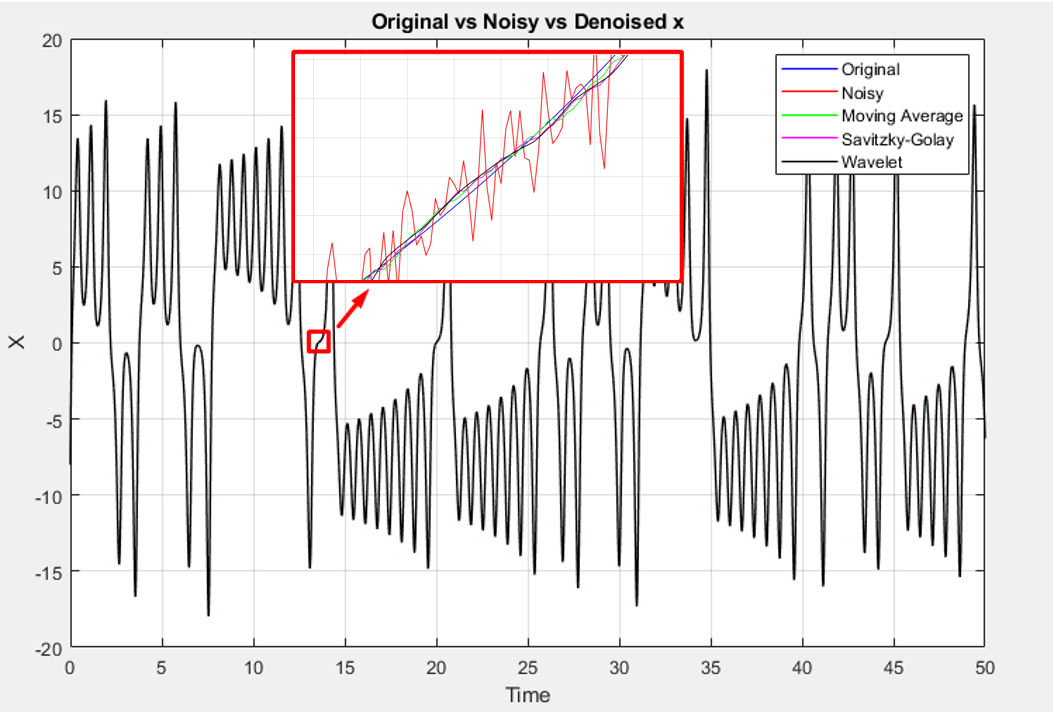
\includegraphics[width=0.7\linewidth]{Figure1}
		\caption{Graph of \(x(t)\) for the Lorenz system with added noise and after denoising, including a zoomed-in portion to highlight subtle differences.}
		\label{fig:figure2}
	\end{figure}
	
	\begin{figure}[htbp]
		\centering
		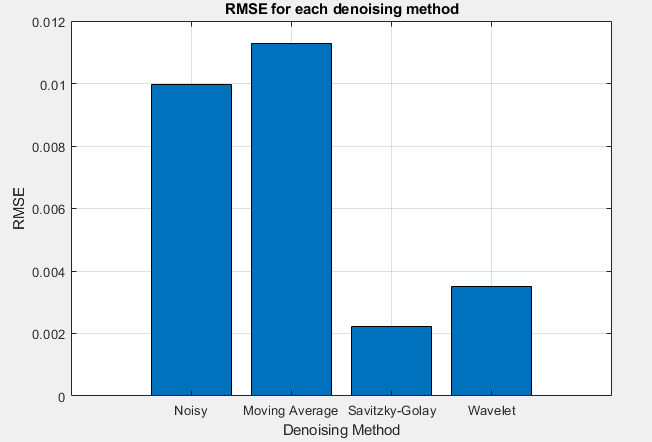
\includegraphics[width=0.7\linewidth]{Figure2}
		\caption{Bar chart of RMSE for different denoising methods. Lower RMSE indicates better alignment with the true (noise-free) signal.}
		\label{fig:figure3}
	\end{figure}
	
	From Figure~\ref{fig:figure3}, Savitzky-Golay and Wavelet Denoising substantially lower error than the noisy dataset itself. Interestingly, the simple Moving Average filter performs worse on average than leaving the data noisy. This motivates focusing on Savitzky-Golay and Wavelet Denoising in future research.
	
	\subsection{Denoised HAVOK Reconstructions}
	With the same Gaussian noise settings, we now feed the denoised signals to the HAVOK pipeline. Figure~\ref{fig:figure4} compares the delay-embedded attractors from noisy vs. denoised data, while Figure~\ref{fig:figure5} shows the time evolution of an error metric (cf.\ Section~2.5) for each approach.
	
	\begin{figure}[htbp]
		\centering
		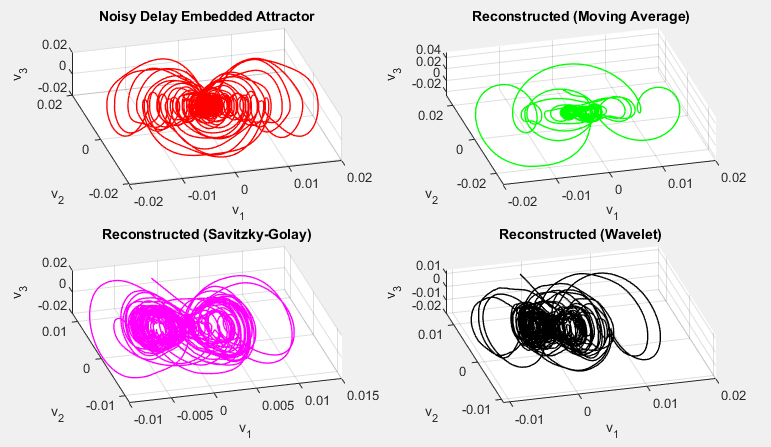
\includegraphics[width=0.7\linewidth]{Figure4}
		\caption{The noisy delay-embedded attractor compared to its denoised version (both using HAVOK). Savitzky-Golay and Wavelet Denoising more closely preserve the two-lobe structure.}
		\label{fig:figure4}
	\end{figure}
	
	\begin{figure}[htbp]
		\centering
		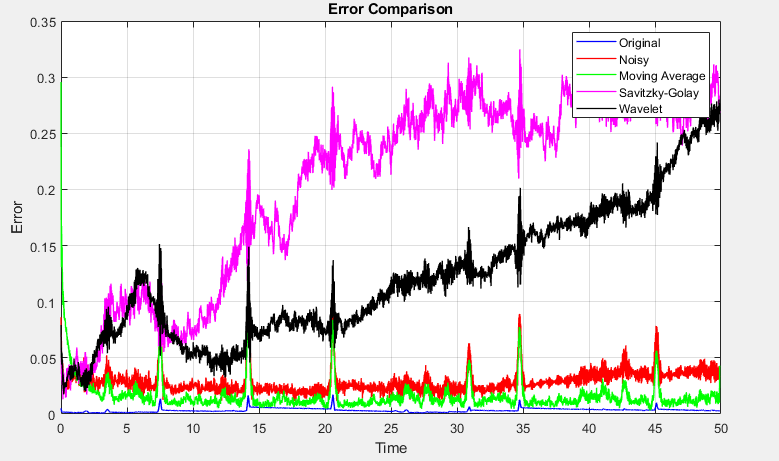
\includegraphics[width=0.7\linewidth]{Figure5}
		\caption{The time evolution of the reconstruction error for each denoising method. Although Savitzky-Golay and Wavelet appear worse by this metric, visual inspection reveals they preserve the Lorenz structure better (see text).}
		\label{fig:figure5}
	\end{figure}
	
	\subsection{Error Measure Revisited}
	We observe that the error metric in Figure~\ref{fig:figure5} often doesn't agree the actual quality of the reconstructed attractors. This occurs because our metric treats all rows in the \(\mathbf{V}\) matrix equally, while HAVOK itself focuses on the most dominant (first ones) modes for reconstruction. Figure~\ref{fig:figure6} illustrates how the first few modes match  closely, but noise takes over the higher modes that are less critical to the main dynamics. Future work will explore more nuanced error measures that weigh modes according to their importance in HAVOK.
	
	\begin{figure}[htbp]
		\centering
		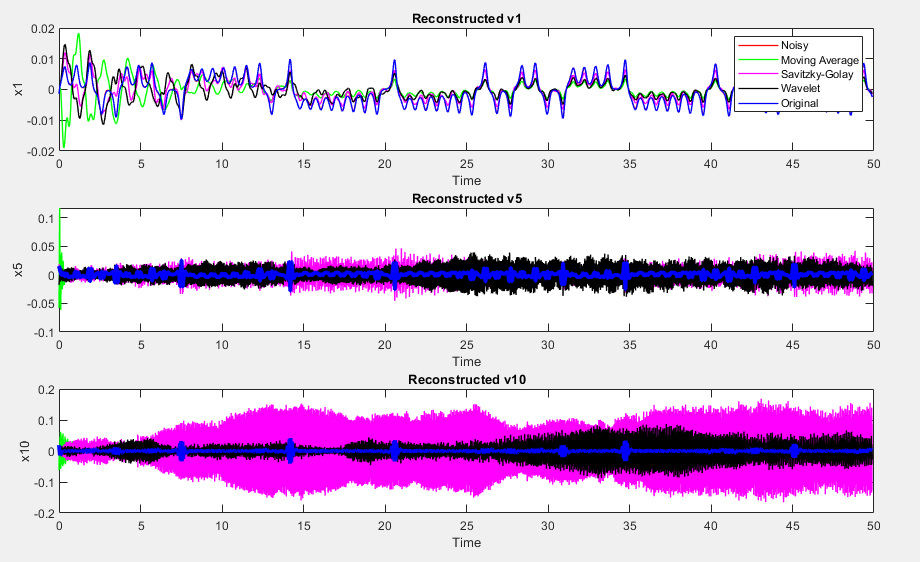
\includegraphics[width=0.7\linewidth]{Figure6}
		\caption{Comparison of the first, fifth, and tenth modes in \(\mathbf{V}\) for different denoising methods. The lower modes match closely, while higher modes exhibit very visible effects of noise.}
		\label{fig:figure6}
	\end{figure}
	
	%--------------------------------------------------
	% 4. DISCUSSION
	%--------------------------------------------------
	\section{Discussion}
	
	\subsection{Investigating the Cause of Poor Performance}
	From Figure~\ref{fig:figure1}, we see that Takens Embedding is not the bottleneck but the linearization from HAVOK is what appears most sensitive to noise. One direction to mitigate this would be to increase \(r\), the number of modes retained, so that small errors do not disproportionately affect the lower-dimensional model, but research is required to confirm it.
	
	\subsection{Noise Removal Performance}
	As shown in Figures~\ref{fig:figure2} and~\ref{fig:figure3}, Savitzky-Golay and Wavelet Denoising are more effective than either leaving the signal noisy or applying a simple Moving Average. Because Wavelet Denoising offers many variable parameters (e.g., wavelet type and thresholds), it presents a rich area for further improvement so that will be my highest area of focus next semester.
	
	\subsection{Denoised Havok Reconstructions}
	Figure~\ref{fig:figure4} demonstrates that Savitzky-Golay and Wavelet Denoising yield significantly clearer attractors with two distinct lobes. However, some noise remains, and improving these filters (especially wavelets) is an ongoing focus for the next semester. A more sophisticated wavelet thresholding strategy or a different wavelet choice might further enhance reconstruction.
	
	\subsection{Error Measure}
	Figure~\ref{fig:figure5} highlights a key issue: a single RMSE measure across all modes of \(\mathbf{V}\) can be misleading. HAVOK prioritizes dominant modes, meaning that less important modes (which may contain mostly noise) can inflate the error without affecting overall attractor fidelity. Thus, a weighted error measure would be more appropriate and the first focus for next year to ensure good comparisons.
	
	%--------------------------------------------------
	% 5. RESEARCH QUESTIONS
	%--------------------------------------------------
	\section{Research Questions}
	Looking ahead, the following questions guide the next phase of this study:
	\begin{enumerate}
		\item How can we effectively remove measurement noise from a chaotic time series while preserving the underlying structure?
		\item To what extent does noise removal improve the accuracy of the HAVOK method for reconstructing the attractor?
		\item How does the HAVOK method, combined with noise-reduced data, improve our ability to predict and model chaotic systems?
		\item What are the limitations of the proposed denoising techniques when applied to different types and levels of noise?
		\item What error measures can we use to better reflect the dominance of lower HAVOK modes?
	\end{enumerate}
	
	%--------------------------------------------------
	% 6. CONCLUSION
	%--------------------------------------------------
	\section{Conclusion}
	In this study, I explored methods for removing noise from chaotic dynamical systems, specifically with of the Lorenz attractor, to improve the accuracy of HAVOK's linear reconstructions. Through the application of three noise reduction techniques-Moving Average, Savitzky-Golay, and Wavelet Denoising—I evaluated their performance in preserving the real chaotic structure while removing as much of the noise (measurement error) as possible.
	
	The results showed that Moving Average was least effective, usually performing even worse than leaving the data noisy. By contrast, Savitzky-Golay and Wavelet Denoising performed significantly better, retaining the attractor’s overall shape and reducing noise levels for the HAVOK procedure. Moreover, we made sure that the main sensitivity to noise lies in the linearization step of HAVOK rather than the Takens Embedding. This suggests possible improvements, such as increasing the number of modes \(r\) to capture the more of the important dynamics.
	
	We also highlighted that the standard RMSE metric across all modes of the \(\mathbf{V}\) matrix is a poor measure of error. Because HAVOK focuses on the most dominant rows, noise in the higher modes can increase error measurements without drastically changing the reconstruction. Future work will focus on developing better error measures and on refining wavelet-based denoising by experimenting with different wavelet types and ways of thresholding.
	
	Finally, these advances will help make data-driven modeling of chaotic systems more robust to noise which will make HAVOK a far more useful method, with potential applications in meteorology, finance, biological systems and many more.
	
	%--------------------------------------------------
	% REFERENCES
	%--------------------------------------------------
	\begin{thebibliography}{99}
		
		\bibitem{brunton2017}
		Brunton, S. L., Brunton, B. W., Proctor, J. L., \& Kutz, J. N. (2017).
		\textit{Chaos as an intermittently forced linear system}. Nature Communications.
		
		\bibitem{brunton2015}
		Brunton, S. L., Proctor, J.L., \& Kutz, J. N. (2017).
		\textit{Discovering governing equations from data: Sparse identification of nonlinear dynamical systems}. PNAS.
		
		\bibitem{luo2012}
		Luo, G., \& Zhang, D. (2012). 
		\textit{Wavelet Denoising}. In \textit{Advances in Wavelet Theory and Their Applications in Engineering, Physics and Technology}. IntechOpen. 
		\href{https://doi.org/10.5772/37424}{https://doi.org/10.5772/37424}
		
	\end{thebibliography}
	
\end{document}
